\chapter{Introduction}
Over the last ten years, the electronics industry has exploded. The largest portion of the total worldwide sales is dominated by the MOS market. Composed primarily of memory, micro and logic sales, the total combined MOS revenue contributed approximately 75 percent of the worldwide sales, illustrating the strength of CMOS technology. CMOS technology currently continues to mature, with minimum feature sizes now approaching 10nm. This has resulted in development in process technologies and have allowed design of circuits using devices running at lower currents, lower voltages and at higher unity gain frequencies. This has done signal processing world a great deal of good, resulting in creation of amplifiers with high speed and converters operting under low voltage conditions.

The necessity for high voltage integrated circuits, capable of driving high currents, remains greater than ever before, with countless applications related to emerging technologies. There are numerous applications of high current amplifiers which can be used in any signal processing context involving driving loads which require high current. One of the common applications is in the Current Transformer circuits.

Operational Transconductance Amplifier(OTA) is a building block for most of the analog circuits with linear input-output characteristics. Operational Amplifiers (OP AMP) too are used as a basic building block in implementing a variety of analog applications such as amplifiers, summers, differentiators, integrators, etc to a more complicated applications like Oscillators. 

For more than 50 years, silicon-on-insulator (SOI) technologies have been developed for radiation-hardened military and space applications.  The  use  of  SOI  has  been  motivated  by  the  full dielectric  isolation  of  individual  transistors,  which  prevents
latchup.Many efforts have been made to reduce these parasitic structures and very high levels of radiation hardness have been achieved. In addition, major chip manufacturers are now producing SOI technologies for many nonhardened high performance or low-power applications.

This document describes the design and implementation of such a radiation hard transconductance amplifier, which is used in a DC current transformer. The report is structured as follows: First, the concept of Closed Loop DC Current Transformer is introduced. Then, the theory of the building blocks of the design along with the methodology is provided. After that, the design and implementation of each of these building blocks which was done in Cadence Virtuoso environment is documented in separate chapters. And then the corner simulation results of the design and the conclusion of the thesis work are documented in the subsequent chapters of this document.

\vfill
\clearpage

\section{Novel DC Current Transformer}

DC Current Transformers (DCCTs) are known as  non-intercepting  standard  tools  for online beam current measurement in synchrotrons and storage rings. In general, the measurement principle of commonly used DCCTs is to introduce a modulating AC signal for a pair of ferromagnetic toroid \cite{ndcct_gsi}. Currently a Novel DCCT (NDCCT) based on modern magnetic field sensors is under development at GSI. The closed-loop NDCCT Design can be considered as an extension to the primary design proposed by GSI. A feedback loop was designed to improve the linearity and sensitivity of the NDCCT. Figure.\ref{fig:HRDCCT} shows the closed loop NDCCT structure\cite{hrdcct}. The main objective is to provide a feedback current that cancels the magnetic field of the ion-beam inside the air gap. This measurement principle is referred to as "Zero-flux" and it is currently used in commercial DCCT.

The change in magnetic field will be sensed by the TMR (Tunneling Magneto Resistance) sensor and it produces a small volage. This voltage is amplified by a Voltage amplifier and is converted to a feedback current $I_{FB}$ by the OTA. This current flows through the N turns winding wire terminated with a resistive load. And this is where the thesis work fits in. The main task of the OTA is to amplify a small AC voltage and produce a high current that drives a resistive load and cancels the magnetic field of the ion-beam.

As a proof of concept, this Closed Loop NDCCT was constructed with the commercial OTAs OPA860 and OPA861 with multiple of those ICs in parallel to get a good understanding of the requirements from the OTA in terms of specifications and results with a dual bipolar power supply of 5V and -5V.

\begin{figure} [H]
\centering
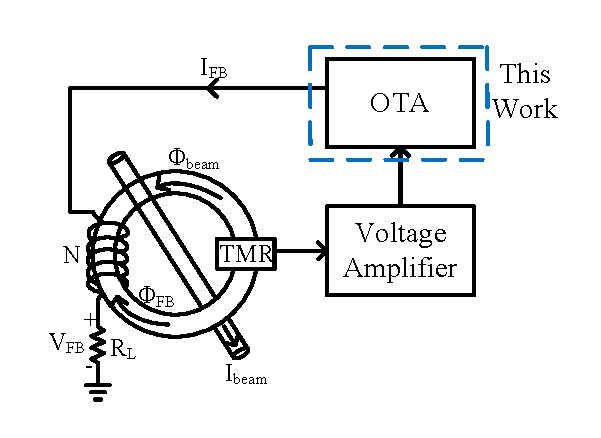
\includegraphics[scale=1]{Figures/System_Level/HRDCCT.pdf}
\caption{Closed Loop Novel-DC Current Transformer}
\label{fig:HRDCCT}
\end{figure}

\vfill
\clearpage

\section{Specification}
As the transconductance amplfier will be a part of the NDCCT, the specifications of the design were obtained from the commercial OTAs OPA860 and OPA861 which were used on a PCB with a power supply of 5V and -5V. Since the OTA is being targetted for multiple applications, it is important to make the design programmable. The specifications are tabulated in detail in Table.\ref{tab:Specs}

\begin{table} [H]
\centering
\begin{tabular}{@{}cc@{}}
\toprule
Parameter						& Value/Specification		\\ \midrule
Circuit Design					& Programmable via I/V/external R or C			\\
Transconductance Gain(Gm)		& 75 .. 140 mA/V			\\
Linear Input Voltage Range		& $\pm$200 mV				\\
Output Current Range			& $\pm$15 mA .. $\pm$30 mA	\\
Bandwidth						& 10 MHz					\\
Slew Rate						& $\pm$900 V/$\mu$s			\\
Rise/Fall time					& 4.4 ns					\\
Input Referred Noise			& 3 nV/$\sqrt{Hz}$ @few KHz	\\
Input Impedance					& 0.5 M$\Omega$				\\
Output Impedance				& 55 K$\Omega$				\\
HD2								& Less than -75 dBc			\\
HD3								& Less than -80 dBc			\\
Open Loop Voltage Gain			& Not less than+5 V/V		\\
PSRR							& $\pm$20 $\mu$A/V			\\
\bottomrule
\end{tabular}
\caption{Specifications of the Design}
\label{tab:Specs}
\end{table}

Remarks:
\begin{itemize}
\item Supply Voltage: 5V
\item Max Load Resistance: 1k$\Omega$
\item Technology to be used: XT018 from XFAB
\end{itemize}

\vfill
\clearpage

\section{Technology}

The technology used for designing the building blocks of the system is the XT018 technology. The XT018 series is XFAB's 0.18-micron Module High-voltage SOI CMOS Technology. It combines the benefits of SOI wafers with Deep Trench Isolation and those of a State of the art six metal layers 0.18-micron process\cite{xt018}. This platform is specifically designed for the next generation automotive, industrial and medical applications operating in the temperature range of -40$^0$C to 170$^0$C. The technology related component names used as part of the circuit design are as tabulated in Table.\ref{tab:Components}.

\begin{table} [H]
\centering
\begin{tabular}{@{}ccc@{}}
\toprule
Component	& Name		& Description			\\ \midrule
PMOS		& pe5		& 5V PMOS				\\
NMOS		& ne5		& 5V NMOS				\\
Resistor	& rmtp		& Top Metal Resistor	\\
Capacitor	& cmm4t		& Single MIM Capacitor	\\
\bottomrule
\end{tabular}
\caption{Components used as part of XT018 technology}
\label{tab:Components}
\end{table}

The reason for choosing XT018 to design the amplifier is because SOI technology makes the design radiation hard. Silicon on insulator (SOI) technology refers to the use of a layered silicon-insulator-silicon substrate in place of conventional silicon substrates in semiconductor manufacturing \cite{soi_tech}, especially microelectronics, to reduce parasitic device capacitance, thereby improving performance. SOI-based devices differ from conventional silicon-built devices in that the silicon junction is above an electrical insulator, typically silicon dioxide or sapphire. 

On the other hand, radiation hardening is the act of making electronic components and systems resistant to damage or malfunctions caused by ionizing radiation (particle radiation and high-energy electromagnetic radiation), such as those encountered in outer space and high-altitude flight, around nuclear reactors and particle accelerators, or during nuclear accidents or nuclear warfare \cite{radhard}. Most semiconductor electronic components are susceptible to radiation damage; radiation-hardened components are based on their non-hardened equivalents, with some design and manufacturing variations that reduce the susceptibility to radiation damage. Due to the extensive development and testing required to produce a radiation-tolerant design of a microelectronic chip, radiation-hardened chips tend to lag behind the most recent developments.